% Aberdeen style guide should be followed when using this
% layout. Their template powerpoint slide is used to extract the
% Aberdeen color and logo but is otherwise ignored (it has little or
% no formatting in it anyway).
%
% http://www.abdn.ac.uk/documents/style-guide.pdf

%%%%%%%%%%%%%%%%%%%% Document Class Settings %%%%%%%%%%%%%%%%%%%%%%%%%
% Pick if you want slides, or draft slides (no animations)
%%%%%%%%%%%%%%%%%%%%%%%%%%%%%%%%%%%%%%%%%%%%%%%%%%%%%%%%%%%%%%%%%%%%%%
%Normal document mode
%\documentclass[10pt,compress]{beamer}
%Draft or handout mode
%\documentclass[10pt,compress,handout]{beamer}
\documentclass[10pt,compress,handout,ignorenonframetext]{beamer} 
\usepackage{xcolor}

\newlength{\overwritelength}
\newlength{\minimumoverwritelength}
\setlength{\minimumoverwritelength}{1cm}
\newcommand{\overwrite}[3][red]{%
  \settowidth{\overwritelength}{$#2$}%
  \ifdim\overwritelength<\minimumoverwritelength%
    \setlength{\overwritelength}{\minimumoverwritelength}\fi%
  \stackrel
    {%
      \begin{minipage}{\overwritelength}%
        \color{#1}\centering\small #3\\%
        \rule{1pt}{9pt}%
      \end{minipage}}
    {\colorbox{#1!50}{\color{black}$\displaystyle#2$}}}


%%%%%%%%%%%%%%%%%%%% General Document settings %%%%%%%%%%%%%%%%%%%%%%%
% These settings must be set for each presentation
%%%%%%%%%%%%%%%%%%%%%%%%%%%%%%%%%%%%%%%%%%%%%%%%%%%%%%%%%%%%%%%%%%%%%%
\newcommand{\shortname}{Dr Jeff Gomes} 
\newcommand{\fullname}{Dr Jeff Gomes}
\institute{School of Engineering}
\newcommand{\emailaddress}{}%{jefferson.gomes@abdn.ac.uk}
\newcommand{\logoimage}{./FigBanner/UoAHorizBanner}
\title{Computational Fluid Dynamics (EG501V)}
\subtitle{Introduction to Turbulence}
\date[]{}


%%%%%%%%%%%%%%%%%%%% Template settings %%%%%%%%%%%%%%%%%%%%%%%%%%%%%%%
% You shouldn't have to change below this line, unless you want to.
%%%%%%%%%%%%%%%%%%%%%%%%%%%%%%%%%%%%%%%%%%%%%%%%%%%%%%%%%%%%%%%%%%%%%%
\usecolortheme{whale}
\useoutertheme{infolines}

% Use the fading effect for items that are covered on the current
% slide.
\beamertemplatetransparentcovered

% We abuse the author command to place all of the slide information on
% the title page.
\author[\shortname]{%
  \fullname\\\ttfamily{\emailaddress}
}


%At the start of every section, put a slide indicating the contents of the current section.
\AtBeginSection[] {
  \begin{frame}
    \frametitle{Section Outline}
    \tableofcontents[currentsection]
  \end{frame}
}

% Allow the inclusion of movies into the Presentation! At present,
% only the Okular program is capable of playing the movies *IN* the
% presentation.
\usepackage{multimedia}
\usepackage{animate}

%% Handsout -- comment out the lines below to create handstout with 4 slides in a page with space for comments
\usepackage{handoutWithNotes}

\mode<handout>
{
\usepackage{pgf,pgfpages}

\pgfpagesdeclarelayout{2 on 1 boxed with notes}
{
\edef\pgfpageoptionheight{\the\paperheight} 
\edef\pgfpageoptionwidth{\the\paperwidth}
\edef\pgfpageoptionborder{0pt}
}
{
\setkeys{pgfpagesuselayoutoption}{landscape}
\pgfpagesphysicalpageoptions
    {%
        logical pages=4,%
        physical height=\pgfpageoptionheight,%
        physical width=\pgfpageoptionwidth,%
        last logical shipout=2%
    } 
\pgfpageslogicalpageoptions{1}
    {%
    border code=\pgfsetlinewidth{1pt}\pgfstroke,%
    scale=1,
    center=\pgfpoint{.25\pgfphysicalwidth}{.75\pgfphysicalheight}%
    }%
\pgfpageslogicalpageoptions{2}
    {%
    border code=\pgfsetlinewidth{1pt}\pgfstroke,%
    scale=1,
    center=\pgfpoint{.25\pgfphysicalwidth}{.25\pgfphysicalheight}%
    }%
\pgfpageslogicalpageoptions{3}
    {%
    border shrink=\pgfpageoptionborder,%
    resized width=.7\pgfphysicalwidth,%
    resized height=.5\pgfphysicalheight,%
    center=\pgfpoint{.75\pgfphysicalwidth}{.29\pgfphysicalheight},%
    copy from=3
    }%
\pgfpageslogicalpageoptions{4}
    {%
    border shrink=\pgfpageoptionborder,%
    resized width=.7\pgfphysicalwidth,%
    resized height=.5\pgfphysicalheight,%
    center=\pgfpoint{.75\pgfphysicalwidth}{.79\pgfphysicalheight},%
    copy from=4
    }%

\AtBeginDocument
    {
    \newbox\notesbox
    \setbox\notesbox=\vbox
        {
            \hsize=\paperwidth
            \vskip-1in\hskip-1in\vbox
            {
                \vskip1cm
                Notes\vskip1cm
                        \hrule width\paperwidth\vskip1cm
                    \hrule width\paperwidth\vskip1cm
                        \hrule width\paperwidth\vskip1cm
                    \hrule width\paperwidth\vskip1cm
                        \hrule width\paperwidth\vskip1cm
                    \hrule width\paperwidth\vskip1cm
                    \hrule width\paperwidth\vskip1cm
                    \hrule width\paperwidth\vskip1cm
                        \hrule width\paperwidth
            }
        }
        \pgfpagesshipoutlogicalpage{3}\copy\notesbox
        \pgfpagesshipoutlogicalpage{4}\copy\notesbox
    }
}
}

%\pgfpagesuselayout{2 on 1 boxed with notes}[letterpaper,border shrink=5mm]
%\pgfpagesuselayout{2 on 1 boxed with notes}[letterpaper,border shrink=5mm]

%%%%% Color settings
\usepackage{color}
%% The background color for code listings (i.e. example programs)
\definecolor{lbcolor}{rgb}{0.9,0.9,0.9}%
\definecolor{UoARed}{rgb}{0.64706, 0.0, 0.12941}
\definecolor{UoALight}{rgb}{0.85, 0.85, 0.85}
\definecolor{UoALighter}{rgb}{0.92, 0.92, 0.92}
\setbeamercolor{structure}{fg=UoARed} % General background and higlight color
\setbeamercolor{frametitle}{bg=black} % General color
\setbeamercolor{frametitle right}{bg=black} % General color
\setbeamercolor{block body}{bg=UoALighter} % For blocks
\setbeamercolor{structure}{bg=UoALight} % For blocks
% Rounded boxes for blocks
\setbeamertemplate{blocks}[rounded]

%%%%% Font settings
% Aberdeen requires the use of Arial in slides. We can use the
% Helvetica font as its widely available like so
% \usepackage{helvet}
% \renewcommand{\familydefault}{\sfdefault}
% But beamer already uses a sans font, so we will stick with that.

% The size of the font used for the code listings.
\newcommand{\goodsize}{\fontsize{6}{7}\selectfont}

% Extra math packages, symbols and colors. If you're using Latex you
% must be using it for formatting the math!
\usepackage{amscd,amssymb} \usepackage{amsfonts}
\usepackage[mathscr]{eucal} \usepackage{mathrsfs}
\usepackage{latexsym} \usepackage{amsmath} \usepackage{bm}
\usepackage{amsthm} \usepackage{textcomp} \usepackage{eurosym}
% This package provides \cancel{a} and \cancelto{a}{b} to "cancel"
% expressions in math.
\usepackage{cancel}

\usepackage{comment} 

% Get rid of font warnings as modern LaTaX installations have scalable
% fonts
\usepackage{type1cm} 

%\usepackage{enumitem} % continuous numbering throughout enumerate commands

% For exact placement of images/text on the cover page
\usepackage[absolute]{textpos}
\setlength{\TPHorizModule}{1mm}%sets the textpos unit
\setlength{\TPVertModule}{\TPHorizModule} 

% Source code formatting package
\usepackage{listings}%
\lstset{ backgroundcolor=\color{lbcolor}, tabsize=4,
  numberstyle=\tiny, rulecolor=, language=C++, basicstyle=\goodsize,
  upquote=true, aboveskip={1.5\baselineskip}, columns=fixed,
  showstringspaces=false, extendedchars=true, breaklines=false,
  prebreak = \raisebox{0ex}[0ex][0ex]{\ensuremath{\hookleftarrow}},
  frame=single, showtabs=false, showspaces=false,
  showstringspaces=false, identifierstyle=\ttfamily,
  keywordstyle=\color[rgb]{0,0,1},
  commentstyle=\color[rgb]{0.133,0.545,0.133},
  stringstyle=\color[rgb]{0.627,0.126,0.941}}

% Allows the inclusion of other PDF's into the final PDF. Great for
% attaching tutorial sheets etc.
\usepackage{pdfpages}
\setbeamercolor{background canvas}{bg=}  

% Remove foot note horizontal rules, they occupy too much space on the slide
\renewcommand{\footnoterule}{}

% Force the driver to fix the colors on PDF's which include mixed
% colorspaces and transparency.
\pdfpageattr {/Group << /S /Transparency /I true /CS /DeviceRGB>>}

% Include a graphics, reserve space for it but
% show it on the next frame.
% Parameters:
% #1 Which slide you want it on
% #2 Previous slides
% #3 Options to \includegraphics (optional)
% #4 Name of graphic
\newcommand{\reserveandshow}[4]{%
\phantom{\includegraphics<#2|handout:0>[#3]{#4}}%
\includegraphics<#1>[#3]{#4}%
}

\newcommand{\frc}{\displaystyle\frac}
\newcommand{\red}{\textcolor{red}}
\newcommand{\blue}{\textcolor{blue}}
\newcommand{\green}{\textcolor{green}}
\newcommand{\purple}{\textcolor{purple}}
 

\begin{document}

% Title page layout
\begin{frame}
  \titlepage
  \vfill%
  \begin{center}
    \includegraphics[clip,width=0.8\textwidth]{\logoimage}
  \end{center}
\end{frame}

% Table of contents
\frame{ \frametitle{Slides Outline}
  \tableofcontents
}


%%%%%%%%%%%%%%%%%%%% The Presentation Proper %%%%%%%%%%%%%%%%%%%%%%%%%
% Fill below this line with \begin{frame} commands! It's best to
% always add the fragile option incase you're going to use the
% verbatim environment.
%%%%%%%%%%%%%%%%%%%%%%%%%%%%%%%%%%%%%%%%%%%%%%%%%%%%%%%%%%%%%%%%%%%%%%


%%%%%%%%%%%%%%%%%%%
%%%   SECTION   %%%
%%%%%%%%%%%%%%%%%%%
\section{Introduction}

%%%
%%% Slide
%%%
\begin{frame}
 \frametitle{Motivation}

   \begin{figure}%
    \begin{center}
     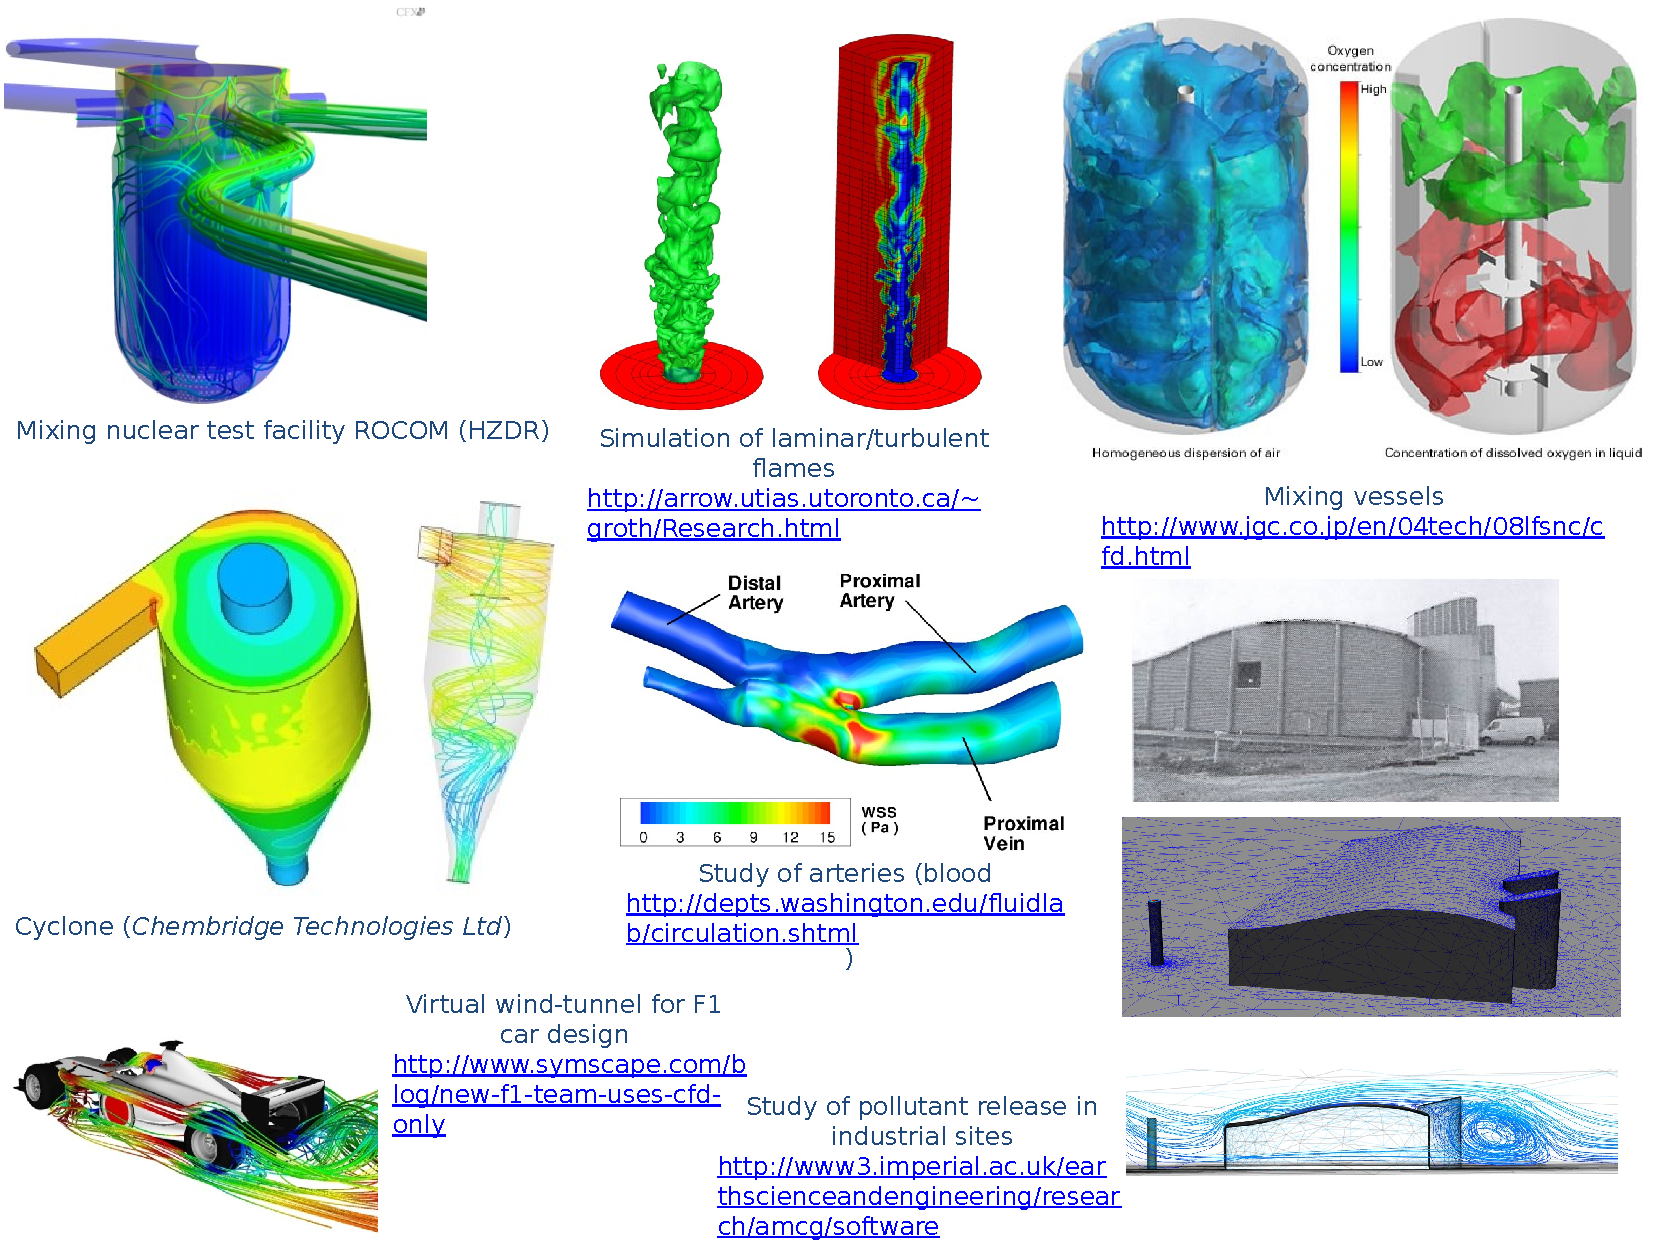
\includegraphics[width=12.cm, height=7.8cm, clip]{./Figs/SpecificIndustrialEnvironmentalApplication2}
    \end{center}
%\caption{XX}
   \end{figure}    

\end{frame}
 
%%%
%%% Slide
%%%
\begin{frame}
 \frametitle{Motivation}

   \begin{figure}%
    \begin{center}
     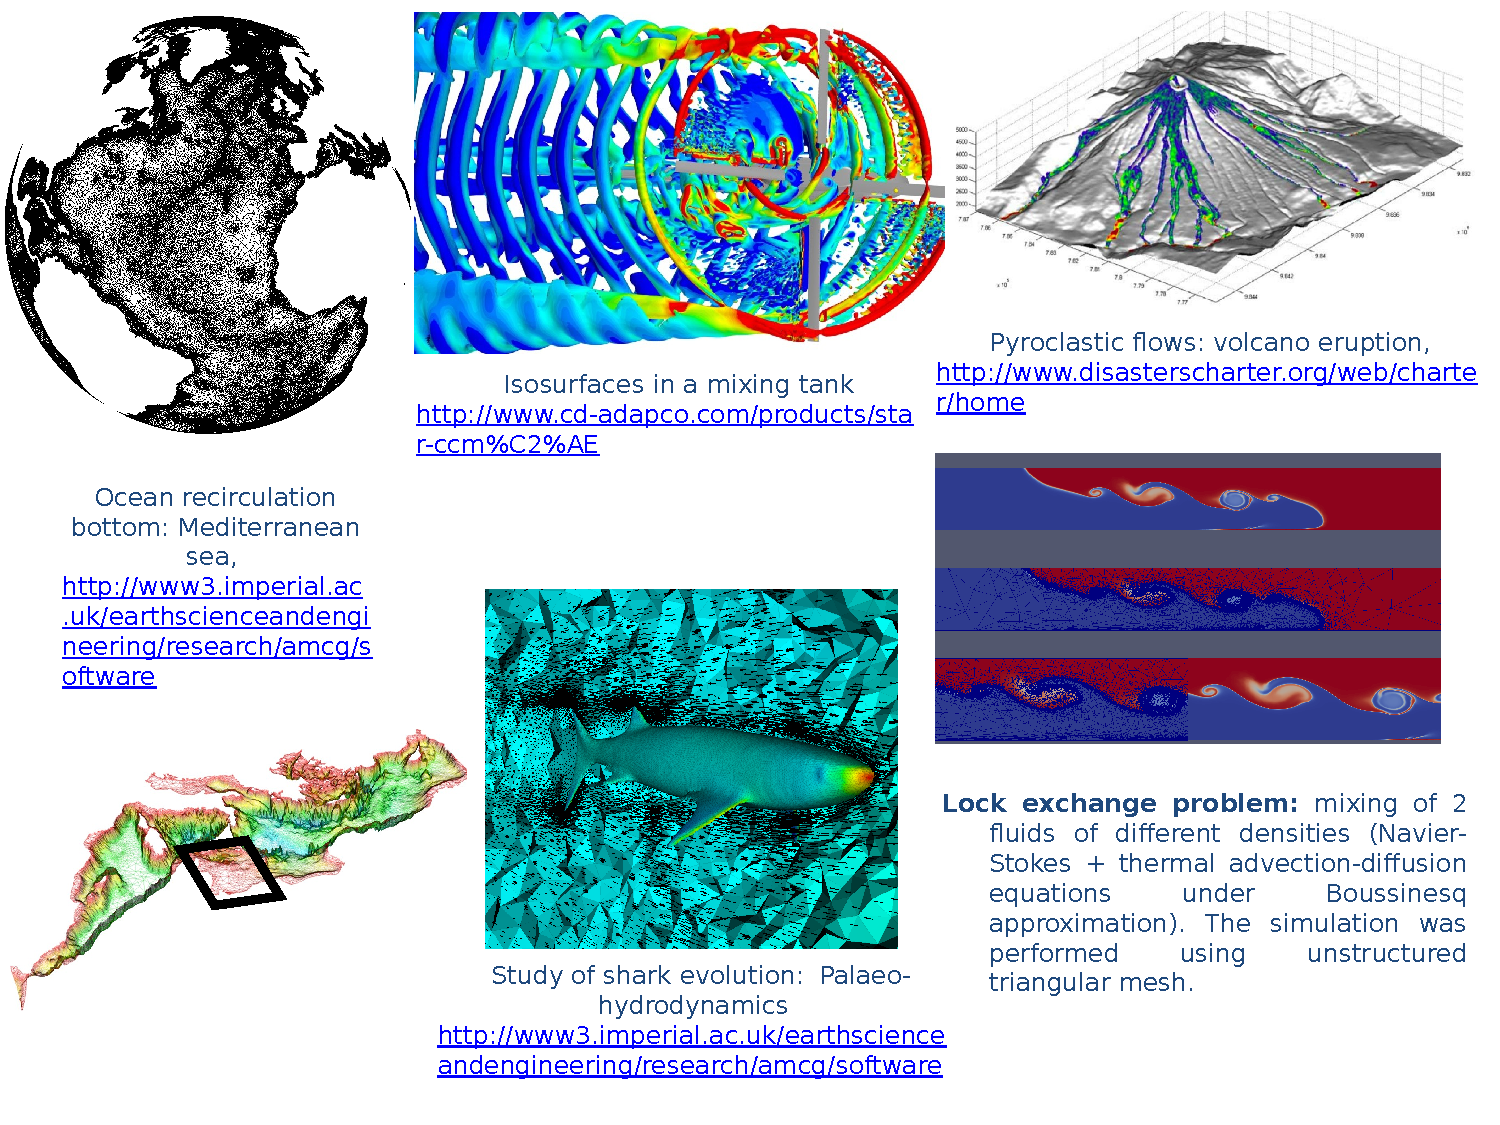
\includegraphics[width=12.cm, height=7.8cm, clip]{./Figs/PostProcessingExamples2.pdf}
    \end{center}
%\caption{XX}
   \end{figure}    

\end{frame}


%%%
%%% Slide
%%%
\begin{frame}
 \frametitle{Objective}
  

   \begin{enumerate}\scriptsize
       \item<1-> From the Navier-Stokes equations for incompressible fluids, we have defined the {\it Reynolds number},
          \visible<1->{\begin{displaymath}
               Re = \frc{\rho \left|u_{ref}\right| L_{ref}}{\mu}
          \end{displaymath}
          that measures the importance of convection and diffusion flow mechanisms.} 
   \end{enumerate}

   \begin{figure}%
    \begin{center}
     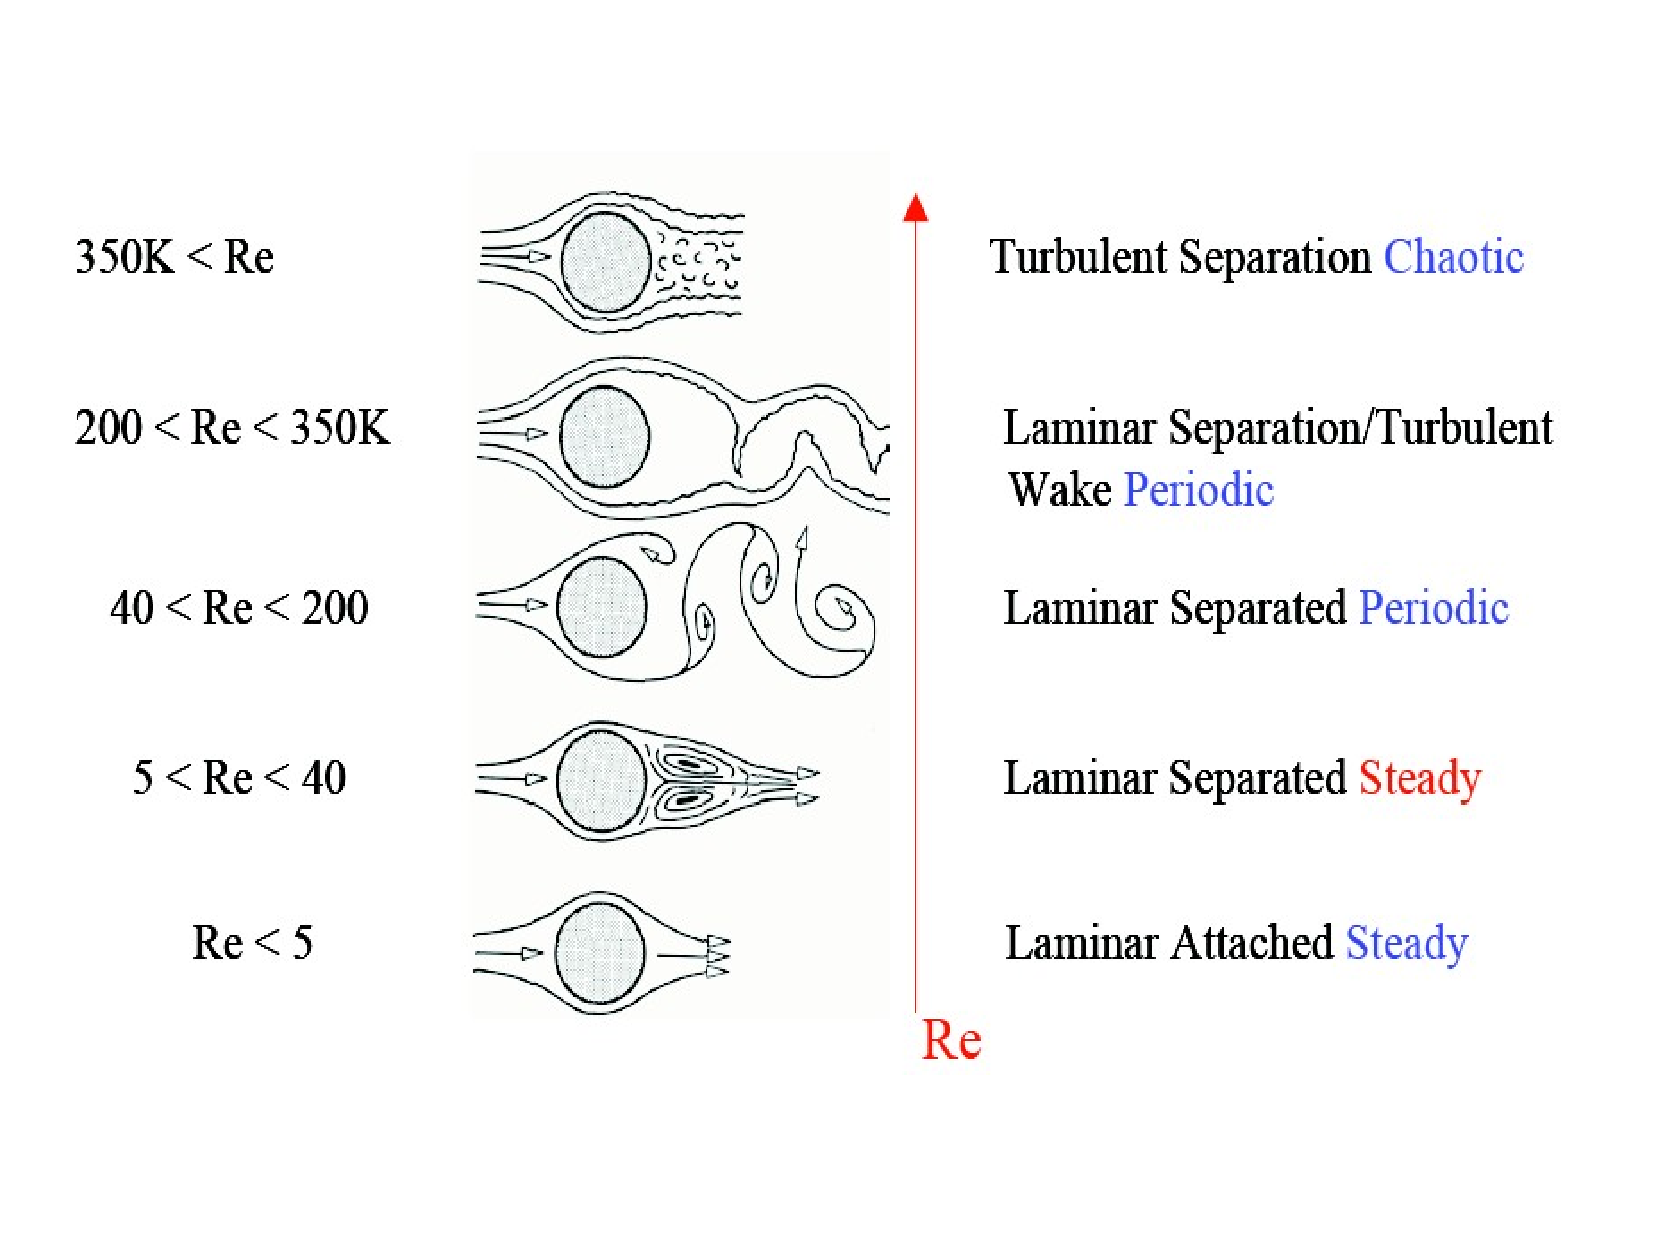
\includegraphics[width=10.cm, height=6.5cm, clip]{./Figs/Transition2Turbulence}
    \end{center}
%\caption{XX}
   \end{figure}  
\end{frame}


%%%
%%% Slide
%%%
\begin{frame}
 \frametitle{Objective}
     \begin{enumerate}\setcounter{enumi}{1}%\scriptsize
       \item<1-> All flows become unstable above a prescribed $Re$;
       \item<1-> At low $Re$ flows are laminar and for high $Re$ flows are turbulent;
       \item<1-> The transition occurs between 2000$\leq Re \leq$ 10$^{6}$;
       \item<2-> Laminar flow problems can be solved using the conservation equations developed previously;
       \item<2-> However, for turbulent flows, the computational effort involved in solving those for {\it all time and length scales} is prohibitive;
       \item<3-> Thus we need an engineering approach to calculate time-averaged flow fields for turbulent flows.
     \end{enumerate} 
\end{frame}

%%%
%%% Slide
%%%
\begin{frame}
 \frametitle{Example: Pollution dispersion in an industrial site}

   \begin{figure}%
    \begin{center}
     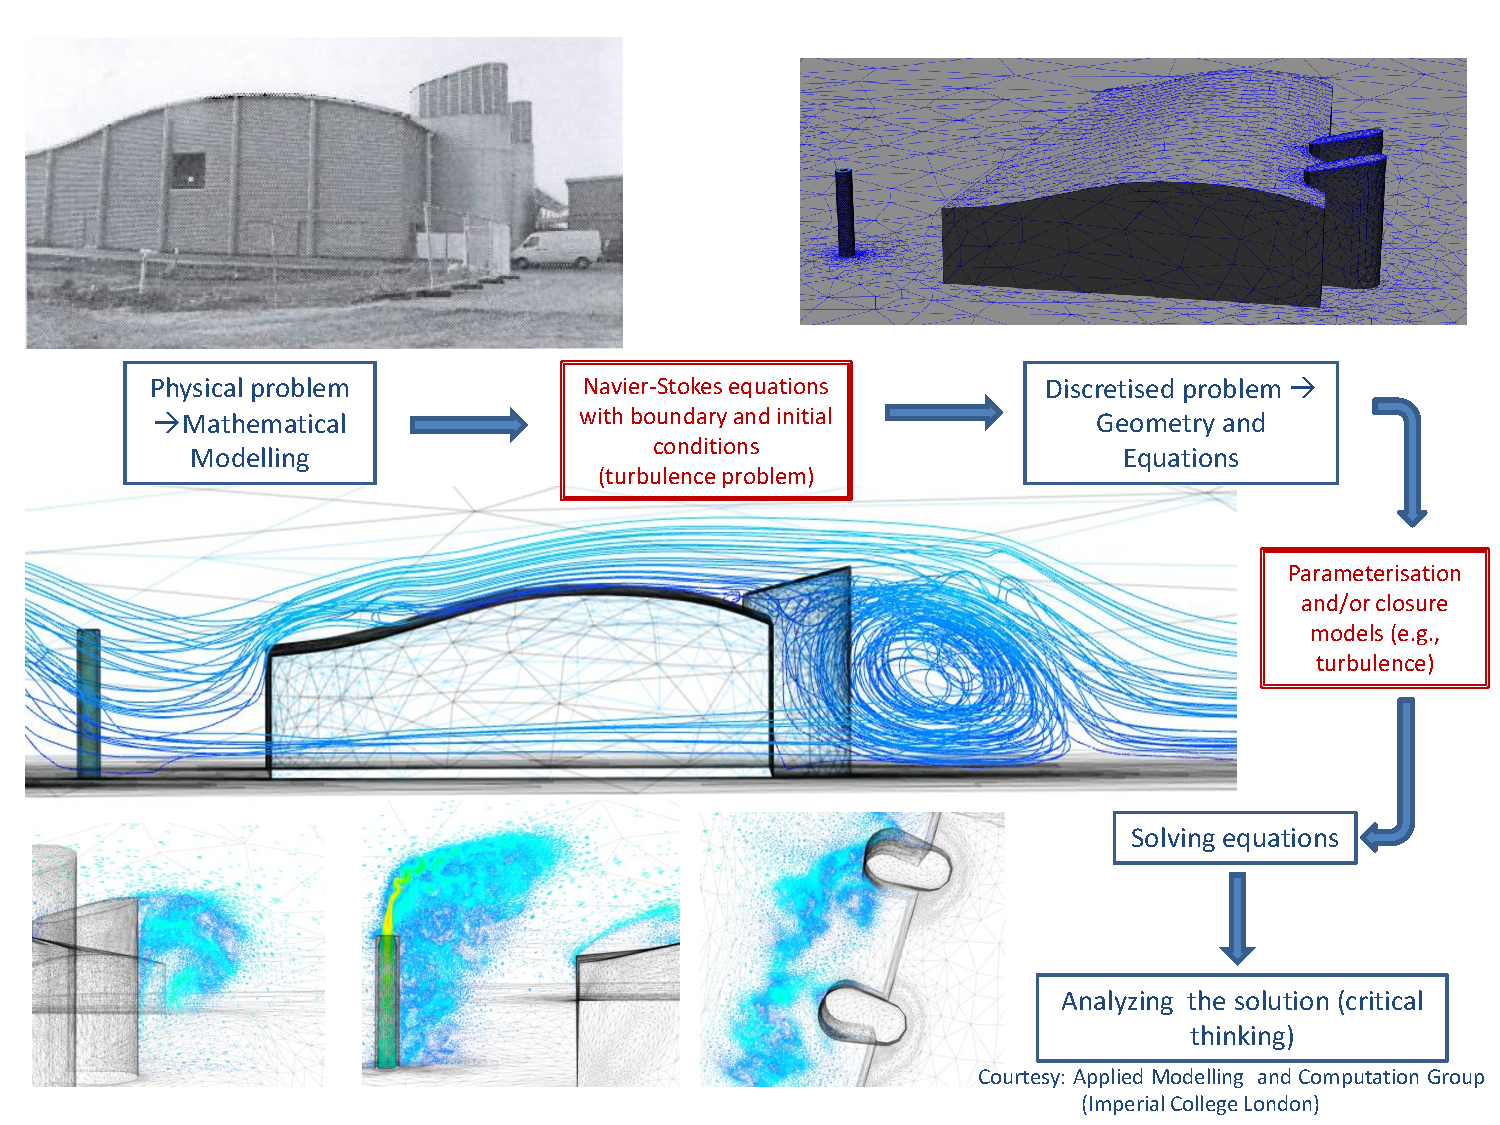
\includegraphics[width=12.cm, height=7.8cm, clip]{./Figs/SpecificIndustrialEnvironmentalApplication.pdf}
    \end{center}
%\caption{XX}
   \end{figure}    
\end{frame}


%%%%
%%%%  SECTION
%%%%

\section{Introduction to Turbulence}

%%%
%%% Slide
%%%
\begin{frame}
 \frametitle{Laminar $\times$ Turbulent Flows}
   \begin{figure}%
    \begin{center}
     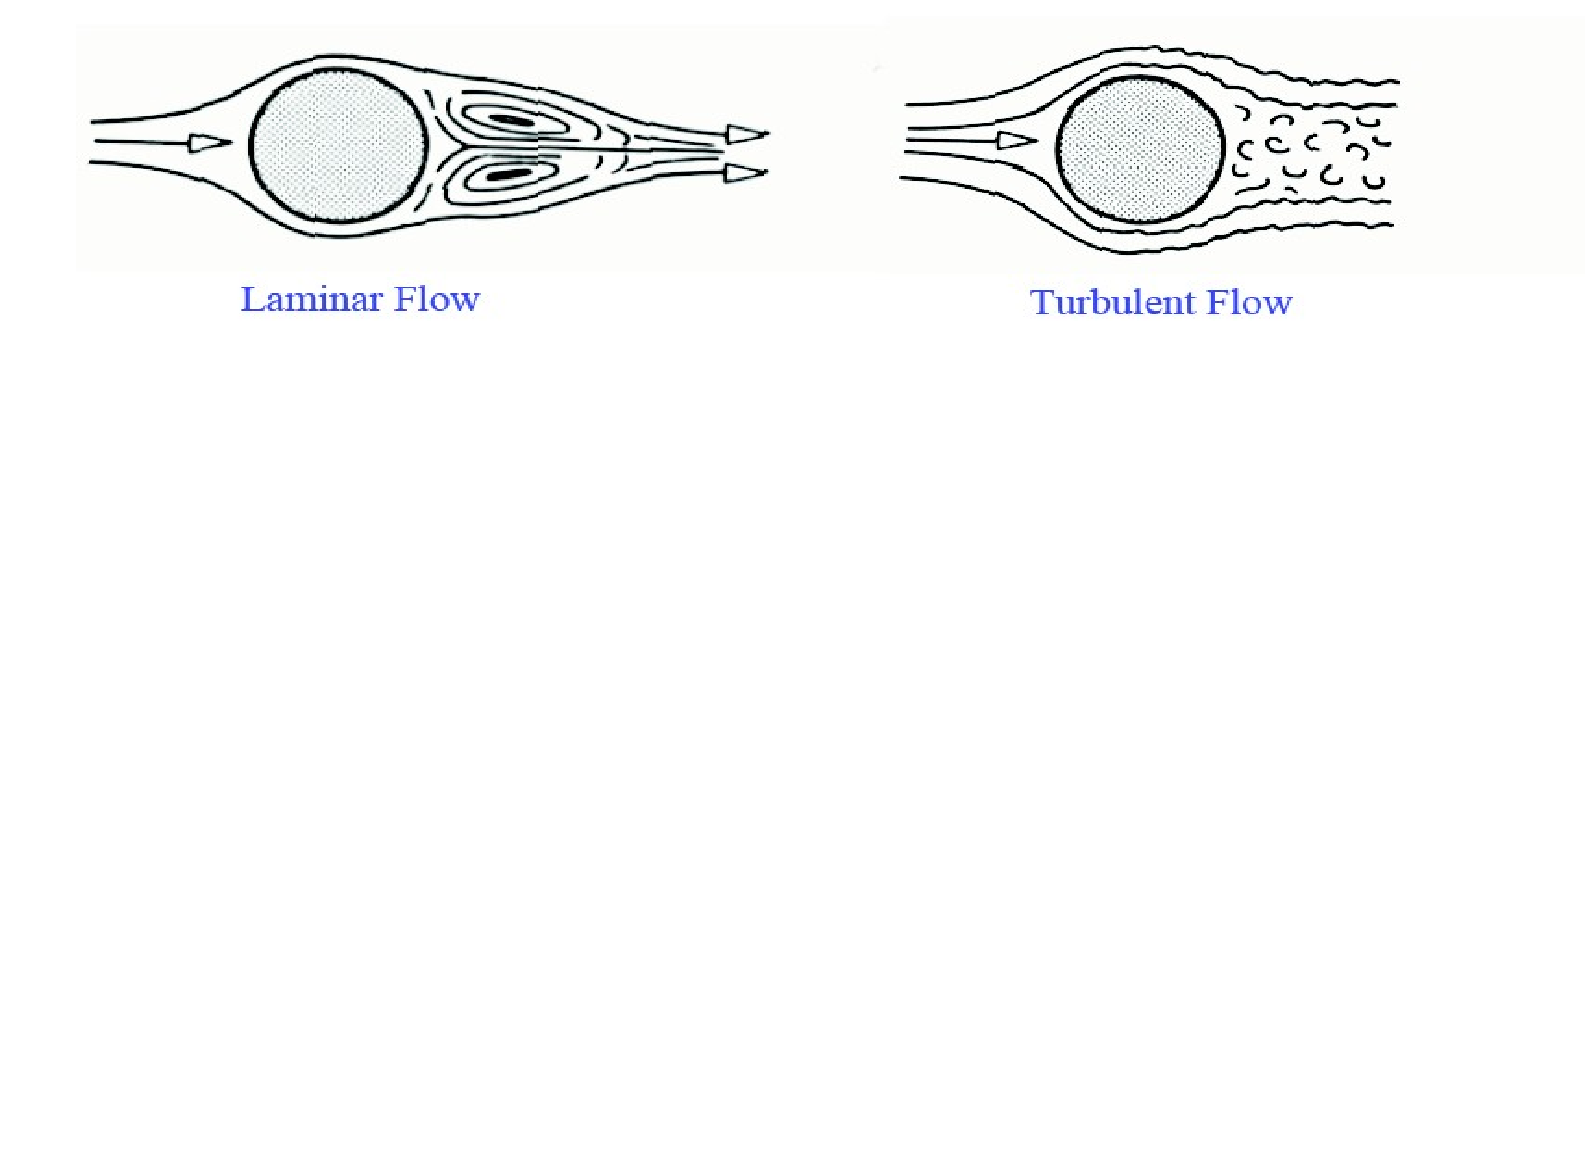
\includegraphics[width=9.cm, height=7cm, clip]{./Figs/Transition2Turbulence2b}
    \end{center}
   \end{figure}    
  \vspace{-5cm}
  \begin{columns}
    \begin{column}[l]{0.5\linewidth}
        The flow is dominated by the object shape and dimension (large scale).
    \end{column}
    \begin{column}[l]{0.5\linewidth}
      The flow is dominated by the object shape and dimension (large scale) and by the motion and evolution of \blue{small eddies} (small scales).
    \end{column}
  \end{columns}

\end{frame}


%%%
%%% Slide
%%%
\begin{frame}
 \frametitle{Introduction to Turbulence}
   \begin{enumerate}
      \item<1-> Turbulence is an unsteady, aperiodic fluid motion in which \blue{all three velocity components} \red{fluctuate}, mixing matter, momentum, and energy;
      \item<1-> Fluid properties under turbulent flows exhibit {\it random} 3-D spatial variations;
      \item<1-> As such, it does present a {\bf strong dependence on initial conditions};
      \item<1-> Turbulent flows contain a wide range of scales (i.e., \blue{edges}).
      \item<2-> Velocity field can be decomposed into \blue{mean} (or average) and \blue{fluctuating} parts (also called {\it Reynolds decomposition}):
         \visible<2->{\begin{equation}
             u_{i} \equiv U_{i} + u^{\prime}_{i}
         \end{equation}
         where $i\in\left\{x, y, z\right\}$. A similar operation can be done for pressure, temperature, concentration etc.}
   \end{enumerate}
\end{frame}

%%%
%%% Slide
%%%
\begin{frame}
 \frametitle{Transition in Boundary-Layer Flow over Flat Plate}
   \begin{figure}%
    \begin{center}
     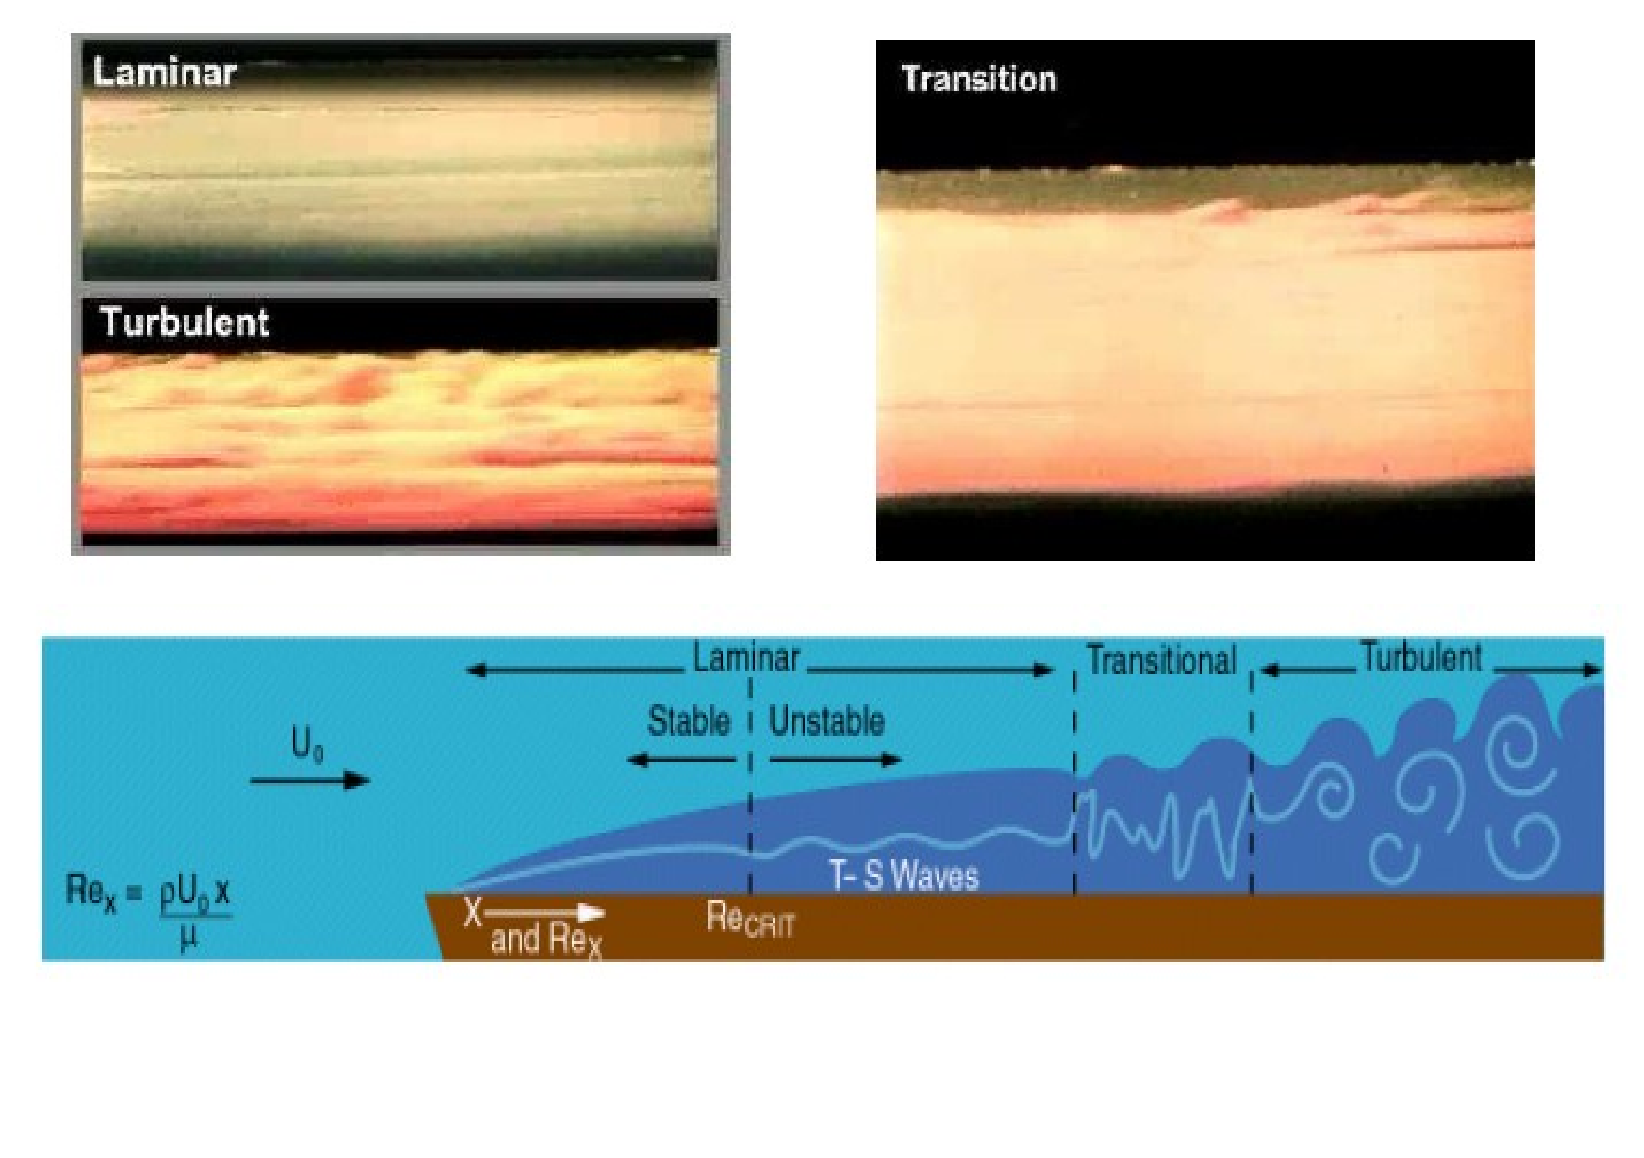
\includegraphics[width=12.cm, height=5cm, clip]{./Figs/Transition2Turbulence3b}
    \end{center}
   \end{figure}  
  \vspace{-1cm}  
  \begin{columns}
    \begin{column}[l]{0.5\linewidth}
       \begin{enumerate}%\scriptsize
           \item<1-> Below $Re_{\text{crit}}$, the flow is laminar and adjacent fluid layers smoothly slide past each other;
           \item<1-> The flow is stable and viscous effects may lead to small disturbances being dissipated;

       \end{enumerate}
    \end{column}
    \begin{column}[l]{0.5\linewidth}
       \begin{enumerate}\setcounter{enumi}{2}%\scriptsize
           \item<1-> Beyond the transition point, $Re_{\text{crit}}$, small disturbances in the flow start to grow.
       \end{enumerate} 
    \end{column}
  \end{columns}

\end{frame}


%%%
%%% Slide
%%%
\begin{frame}
 \frametitle{Transition in Channel Flows}
     \begin{enumerate}%\scriptsize
        \item<1-> Instability and turbulence is also seen in internal flows (e.g., channels and ducts).
        \item<1-> $Re$ may be considered constant throughout the pipe as a function of the fluid properties, flow rare and characteristic diameter;
        \item<2-> Three flow regimes may be found:
            \begin{enumerate}
                \item<2-> $Re < 2200$: Laminar flow;
                \item<2-> $Re = 2200$: Flow alternates between laminar and turbulent;
                \item<2-> $Re > 2200$: Fully turbulent flow.
            \end{enumerate}
       \end{enumerate}

\end{frame}

%%%%%%%%%%%%%%%%%%%
%%%   SECTION   %%%
%%%%%%%%%%%%%%%%%%%
\section{Turbulence Modelling}

%%%
%%% SUBSECTION
%%%
\subsection{Characteristics}

%%%
%%% Slide
%%%
\begin{frame}
 \frametitle{Characteristics of Turbulent Flows}
   \begin{enumerate}
      \item<1-> Irregularity or randomness: Turbulent flows are often described statistically;
      \item<1-> Turbulent flows are always {\it chaotic};
      \item<1-> The \blue{diffusivity} of turbulence causes rapid mixing and increased rates of momentum, heat, and mass transfer. %A flow that looks random but does not exhibit the spreading of velocity fluctuations through the surrounding fluid is not turbulent. If a flow is chaotic, but not diffusive, it is not turbulent. The trail left behind a jet plane that seems chaotic, but does not diffuse for miles is then not turbulent.
      \item<1-> Turbulent flows always occur at high $Re$; they are caused by the {\it complex interaction between the viscous terms and the inertia terms in the momentum equations};
      \item<1-> Turbulent flows are \blue{rotational}, i.e., they have non-zero \blue{vorticity}. Mechanisms such as the stretching of three-dimensional vortices play a key role in turbulence;
      \item<2-> Turbulent flows are \blue{dissipative}, i.e., kinetic energy is converted into heat due to viscous shear stresses; %Turbulent flows die out quickly when no energy is supplied. Random motions that have insignificant viscous losses, such as random sound waves, are not turbulent.
      \item<2-> Turbulence is a \blue{continuum phenomenon} -- even the smallest eddies are significantly larger than the molecular scales; 
      \item<2-> Turbulence is thus governed by the fluid mechanics equations;
      \item<2-> Turbulence \blue{is not a characteristic of the fluid} but rather of the \blue{flow}.
   \end{enumerate}
\end{frame}


%%%
%%% Slide
%%%
\begin{frame}
 \frametitle{Characteristics of Turbulent Flows -- Examples}

   \begin{figure}%
    \begin{center}
     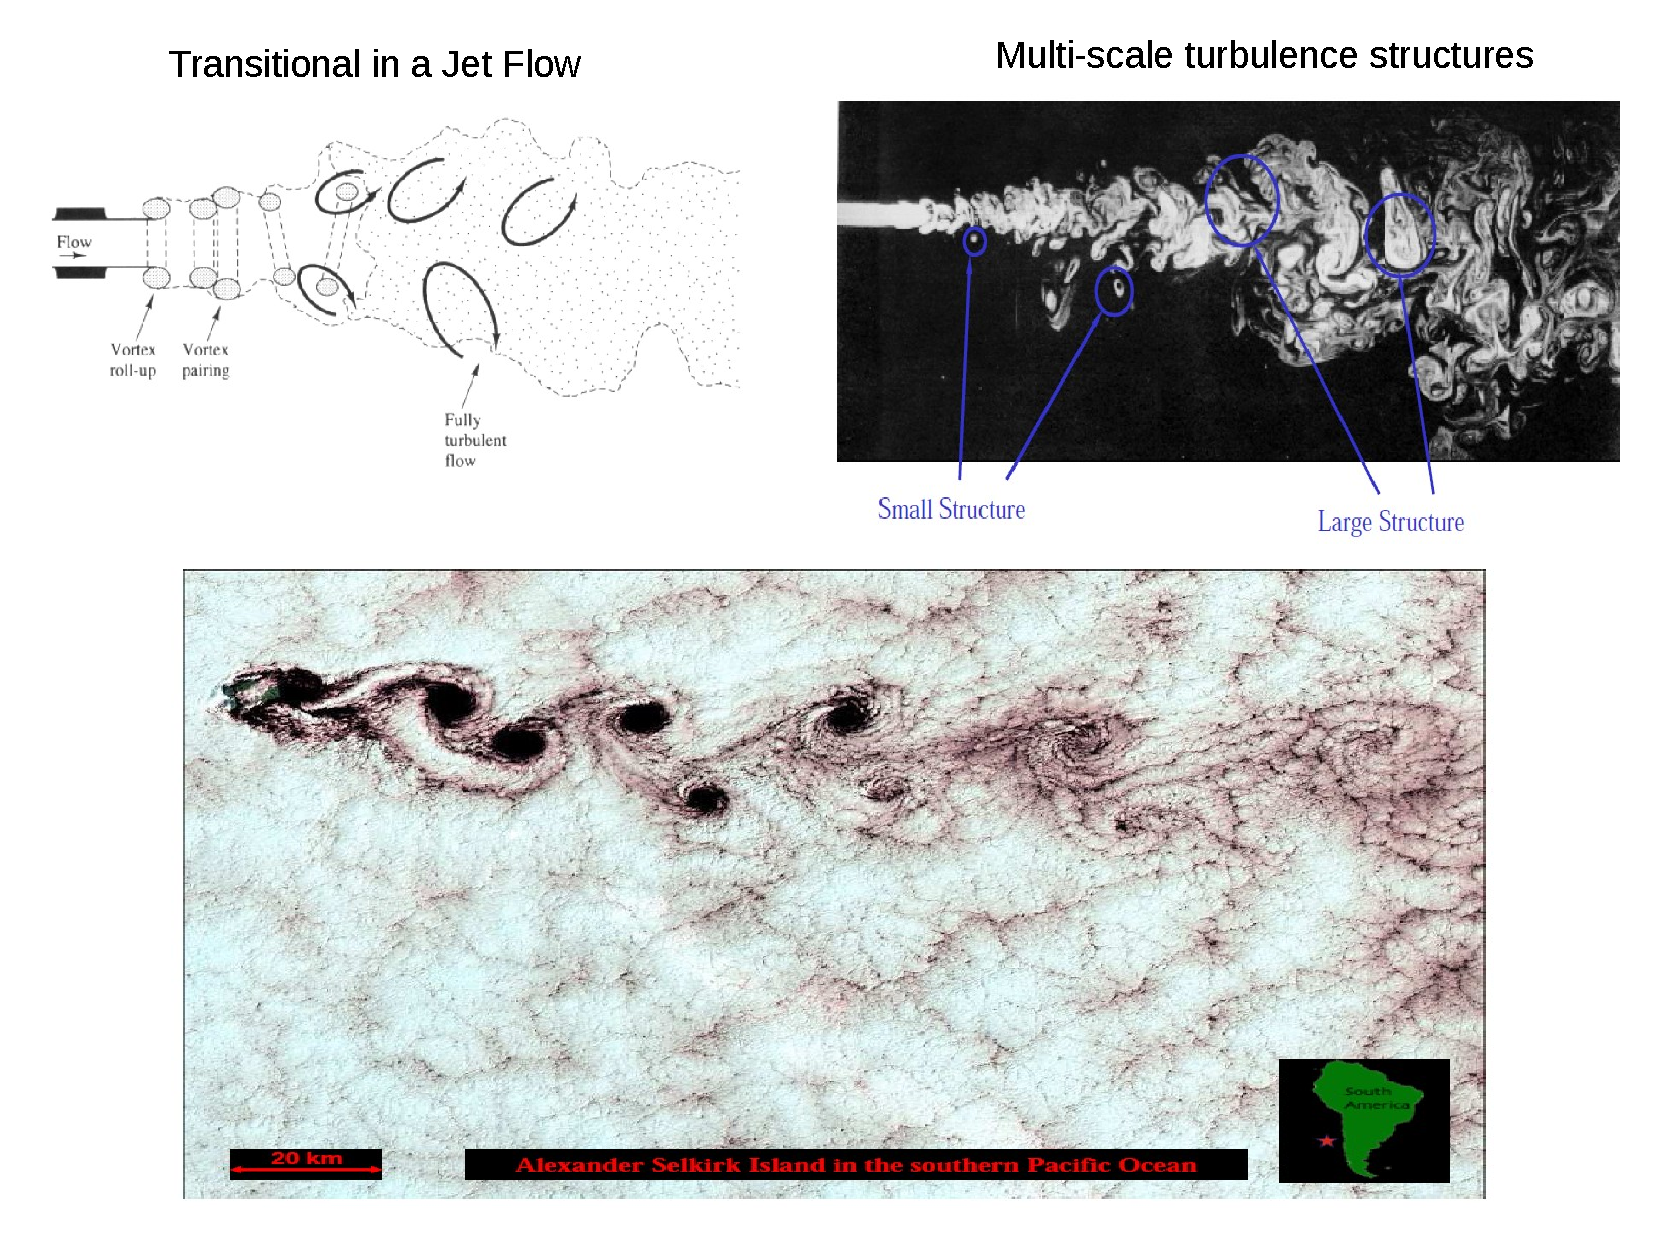
\includegraphics[width=12.cm, height=7.8cm, clip]{./Figs/Turbulence_Examples}
    \end{center}
%\caption{XX}
   \end{figure}    
\end{frame}

%%%
%%% SUBSECTION 
%%%

\subsection{Length-Scale and Vortex}
%%%
%%% Slide
%%%
\begin{frame}
 \frametitle{Kolmogorov Length-Scale}
  \begin{columns}
    \begin{column}[l]{0.5\linewidth}
       \begin{enumerate}%\scriptsize
           \item<1-> $E$ is the energy contained in eddied of wavelength \blue{$\lambda$};
           \item<1-> The energy cascades randomly from large to small scales;
           \item<2-> Length scales:
              \begin{enumerate}%\scriptsize
                  \item<2-> Largest eddies: integral length scale, $k^{3/2}/\epsilon$;
                  \item<2-> Length scales in which turbulence is isotropic: Taylor micro-scale, $\left(15\nu u^{\prime 2}/\epsilon\right)^{1/2}$;
                  \item<2-> Smallest eddies: \blue{Kolmogorov length scale} $\left(\nu^{3}/\epsilon\right)^{1/4}$.
              \end{enumerate}
       \end{enumerate} 
    \end{column}
    \begin{column}[l]{0.5\linewidth}
      \begin{center}
        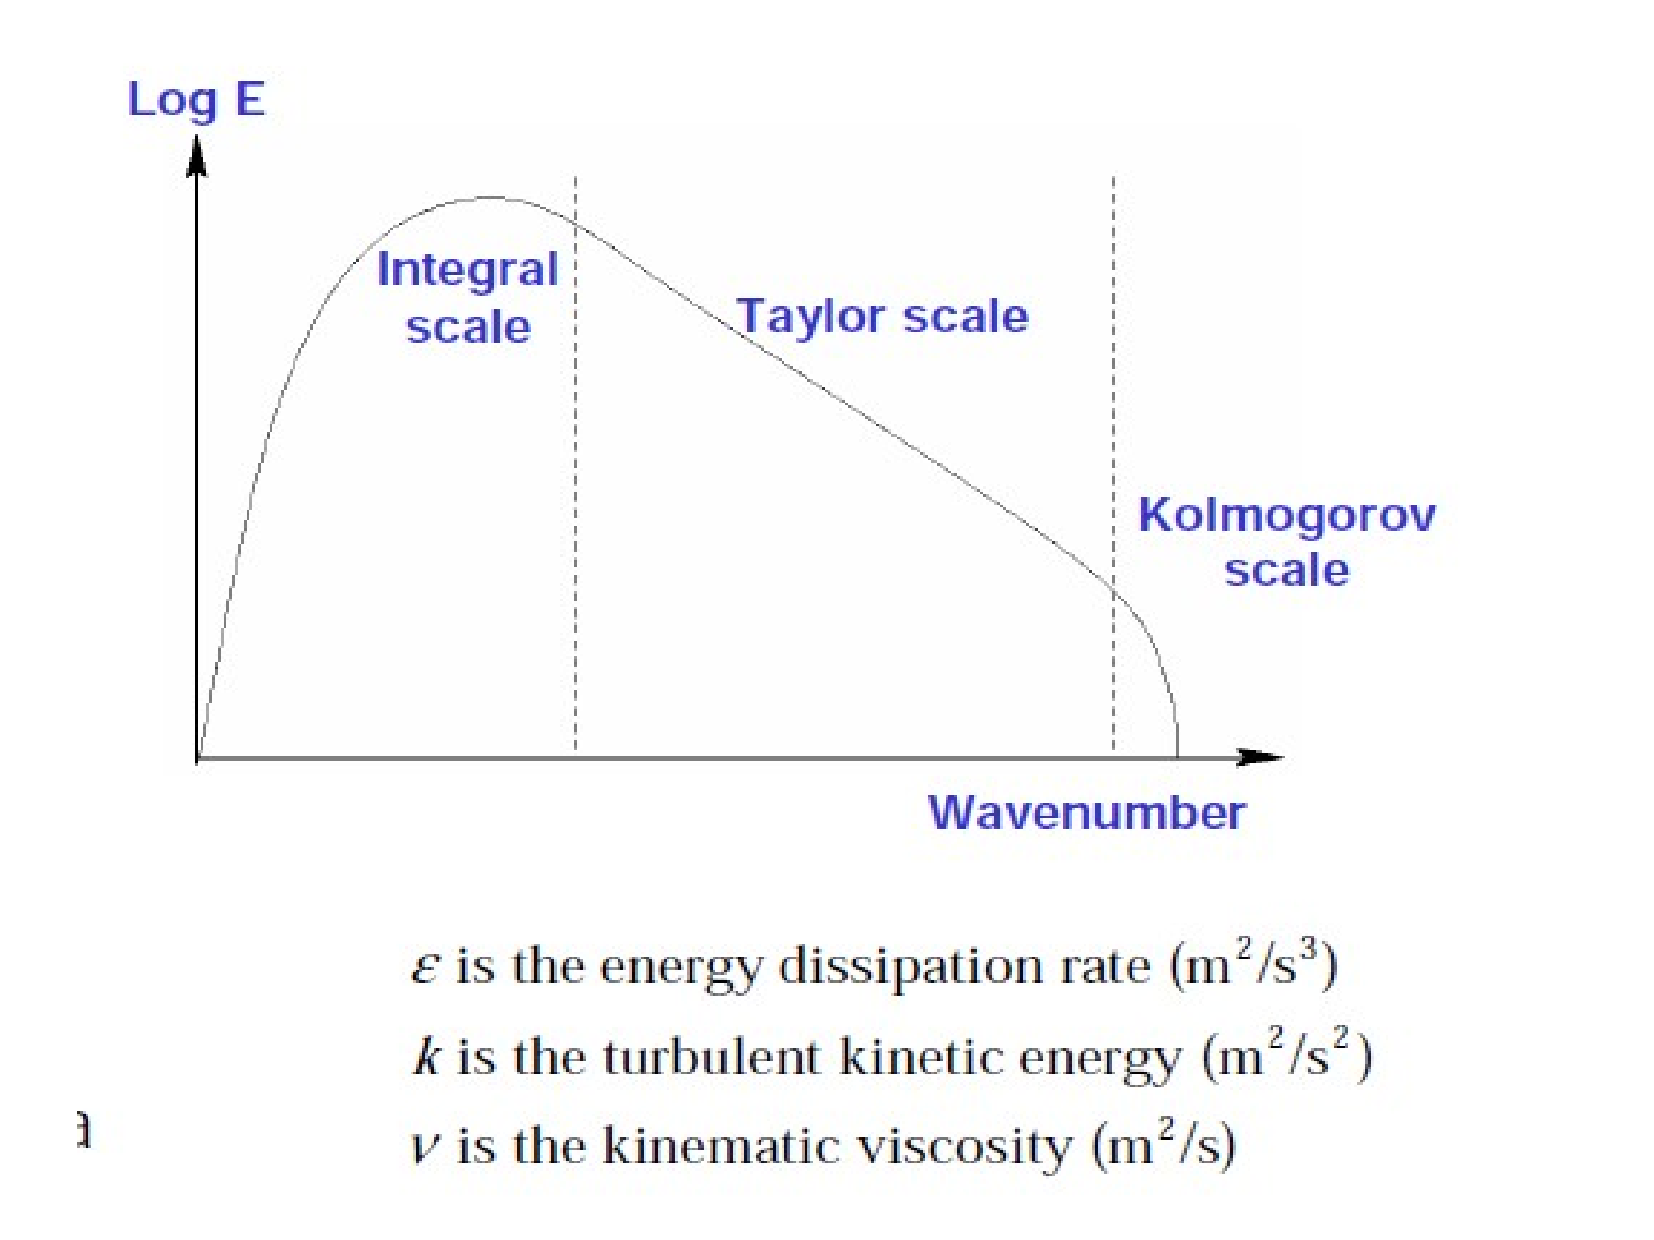
\includegraphics[width=7.cm, height=5cm, clip]{./Figs/Kolmogorov1}
      \end{center}
    \end{column}

  \end{columns}

\end{frame}


%%%
%%% Slide
%%%
\begin{frame}
 \frametitle{Vortices}
    \begin{enumerate}%\scriptsize
       \item<1-> Existence of eddies means  \blue{vorticity} (or \blue{rotation}) along contorted vortex lines;
       \item<1-> As end points of a vortex line move randomly further apart the vortex line increases in length but decreases in diameter;
       \item<1-> Vorticity increases as angular momentum is nearly conserved. Kinetic energy increases at rate equivalent to the work done by large-scale motion that stretches the bundle;
       \item<2-> Viscous dissipation in the smallest eddies converts kinetic energy into thermal energy;
       \item<2-> Vortex-stretching cascade process maintains the turbulence and dissipation is approximately equal to the rate of production of turbulent kinetic energy;
       %\item<2-> Typically energy gets transferred from the large eddies to the smaller eddies. However, sometimes smaller eddies can interact with each other and transfer energy to the (i.e. form) larger eddies, a process known as backscatter.
       \end{enumerate} 
\end{frame}

%%%
%%% SUBSECTION
%%%
\subsection{Reynolds Decomposition}

%%%
%%% Slide
%%%
\begin{frame}
 \frametitle{Flow Properties Decomposition}
    \begin{enumerate}%\scriptsize
       \item<1-> A flow property $\phi$ has a {\it average} $\Phi$ defined as,
          \visible<1->{\begin{displaymath}
            \Phi = \frc{1}{\Delta t}\int\limits_{0}^{\Delta}\phi\left(t\right)dt,
          \end{displaymath}
          where $\Delta t$ is larger than the time-scale of the slowest fluctuation;}
       \item<1-> Leading to           
          \visible<1->{\begin{displaymath}
            \phi = \Phi + \phi^{\prime}
          \end{displaymath}
          where $\phi^{\prime}$ is the fluctuation of $\phi$;}
       \item<2-> Velocity and pressure decomposition:
          \visible<2->{\begin{displaymath}
              u = U + u^{\prime}\hspace{1cm}\text{ and }\hspace{1cm} p = P + p^{\prime},
          \end{displaymath}
          where the average of the fluctuations of are zero, i.e., $\overline{u}^{\prime}=\overline{p}^{\prime}=0$. The {\it overbar} represents time-average quantities, thus $\overline{u}=U$.}
       \item<2-> Turbulent kinetic energy, $k$ is defined as,
          \begin{displaymath}
             k = \frc{1}{2}\left(\overline{u_{x}^{\prime 2}} + \overline{u_{y}^{\prime 2}} + \overline{u_{z}^{\prime 2}}\right)
          \end{displaymath}
       \end{enumerate} 
\end{frame}

%%%
%%% SUBSECTION
%%%
\subsection{RANS Equations}


%%%
%%% Slide
%%%
\begin{frame}
 \frametitle{Direct Numerical Simulation (DNS)}
      \begin{center}
        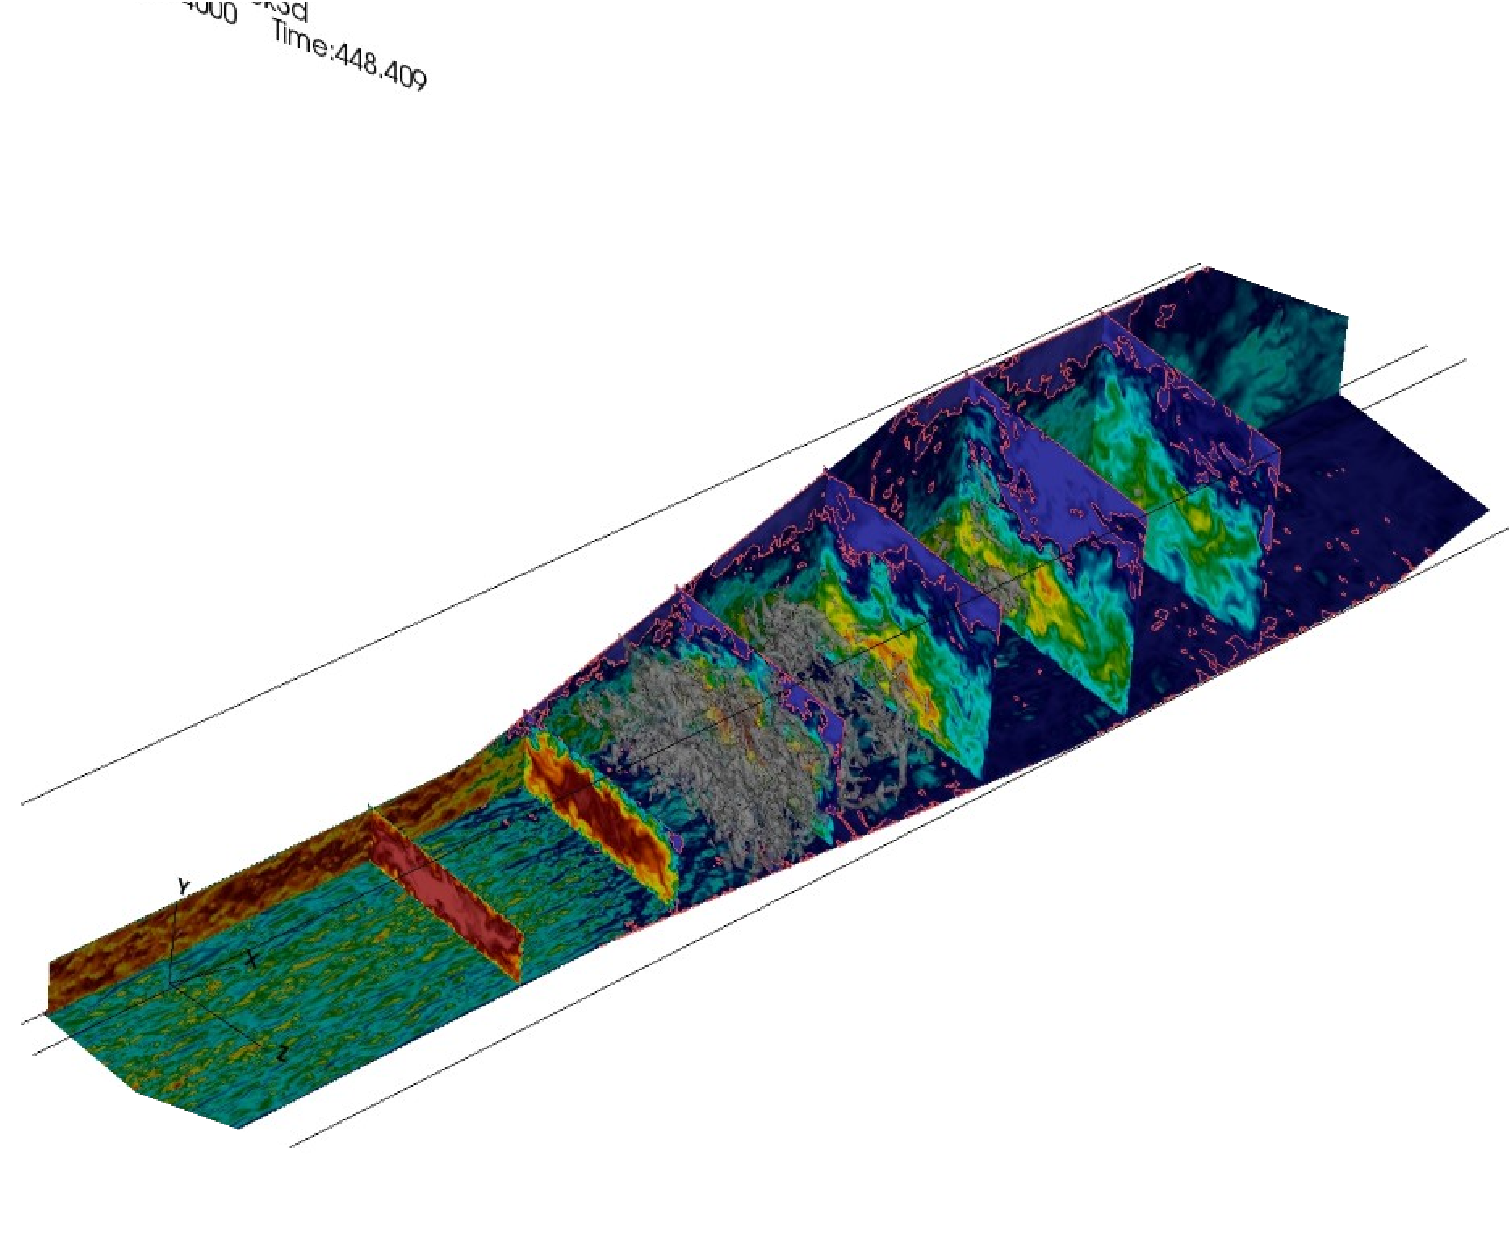
\includegraphics[width=9.cm, height=8cm, clip]{./Figs/DNS_Exampleb}
      \end{center}
\end{frame}


%%%
%%% Slide
%%%
\begin{frame}
 \frametitle{Direct Numerical Simulation (DNS)}
    \begin{enumerate}
       \item<1-> The DNS aims to solve the time-dependent NS equations resolving {\bf ALL} scales (i.e., eddies) for a prescribed time-interval so that fluid properties reach a statistical equilibrium. Thus for a flow with $Re_{\tau}=800$,
          \begin{enumerate}
            \item<1-> Grid requirement: $N\sim\left(Re_{\tau}\right)^{9/4}\sim 10^{7}$;
            \item<1-> Time-step requirement: $\Delta t\sim \left(Re_{\tau}\right)^{1/2}\sim 10^{-5}$;
          \end{enumerate}
          \visible<1->{where $Re_{\tau}=\rho y u_{\tau}/\mu$ and $u_{\tau}=\sqrt{\sigma/\rho}$.}
       \item<2-> DNS can only be used for \underline{\blue{\it relatively low $Re$ and simple geometries}}.
    \end{enumerate} 
\end{frame}

%%%
%%% Slide
%%%
\begin{frame}
 \frametitle{Reynolds-Averaged Navier-Stokes (RANS) Equations}
    \begin{enumerate}
       \item<1-> The NS equations,
          \visible<1->{\begin{eqnarray}
              && \frc{\partial u_{i}}{\partial x_{i}} = 0 \nonumber \\
              && \frc{\partial u_{i}}{\partial t} + u_{j}\frc{\partial u_{i}}{\partial x_{j}} = - \frc{1}{\rho}\frc{\partial p}{\partial x_{i}} + \frc{\partial}{\partial x_{j}}\left(\frc{\mu}{\rho}\frc{\partial u_{i}}{\partial x_{j}}\right) = 0 \nonumber
          \end{eqnarray}}
       \item<2-> Defining Reynolds-averaged quantities,
           \visible<2->{\begin{eqnarray}
              && u_{i}\left(x_{k},t\right) = U_{i}\left(x_{k},t\right) + u^{\prime}\left(x_{k},t\right) \nonumber \\      
              && U_{i}\left(x_{k}\right) = \lim\limits_{T\rightarrow\infty}\frc{1}{T}\int\limits_{0}^{T}u_{i}\left(x_{k},t\right)dt \nonumber
           \end{eqnarray}
           Replacing in the NS equations and averaging,}
    \end{enumerate} 
\end{frame}


%%%
%%% Slide
%%%
\begin{frame}
 \frametitle{Reynolds-Averaged Navier-Stokes (RANS) Equations}
    \begin{enumerate}\setcounter{enumi}{2}%
       \item<1-> Leads to
         \visible<1->{\begin{eqnarray}
               && \frc{\partial U_{i}}{\partial x_{i}} = 0 \label{RANS:Conty} \\
               && \cancelto{0}{\frc{\partial U_{i}}{\partial t}} + U_{j}\frc{\partial U_{i}}{\partial x_{j}} = -\frc{1}{\rho}\frc{\partial P}{\partial x_{i}} + \frc{\partial }{\partial x_{j}}\left(\frc{\mu}{\rho}\frc{\partial U_{i}}{\partial x_{j}}\right)+ \overwrite{\frc{\partial\left(-\overline{u_{i}^{\prime}u_{j}^{\prime}}\right)}{\partial x_{j}}}{Closure problem} \label{RANS:Momentum}
         \end{eqnarray}}
       \item<2-> The transformed momentum equation contain a stress tensor called \blue{Reynolds stress},
          \visible<2->{\begin{displaymath}
              \mathbf{\sigma} = 
              \begin{pmatrix}
                  \sigma_{xx} & \sigma_{xy} & \sigma_{xz} \\
                  \sigma_{yx} & \sigma_{yy} & \sigma_{yz} \\
                  \sigma_{zx} & \sigma_{zy} & \sigma_{zz} \\
              \end{pmatrix} =
              \begin{pmatrix}
                 -\rho\overline{u_{x}^{\prime 2}} & -\rho\overline{u_{x}^{\prime}u_{y}^{\prime}} & - \rho\overline{u_{x}^{\prime}u_{z}^{\prime}} \\ 
                 -\rho\overline{u_{x}^{\prime}u_{y}^{\prime}} & -\rho\overline{u_{y}^{\prime 2}} & - \rho\overline{u_{y}^{\prime}u_{z}^{\prime}} \\ 
                 -\rho\overline{u_{x}^{\prime}u_{z}^{\prime}} & -\rho\overline{u_{y}^{\prime}u_{z}^{\prime}} & - \rho\overline{u_{z}^{\prime 2}} \\ 
              \end{pmatrix}
          \end{displaymath}
          }
    \end{enumerate} 
\end{frame}




%%%
%%% Slide
%%%
\begin{frame}
 \frametitle{Reynolds-Averaged Navier-Stokes (RANS) Equations}
    \begin{enumerate}\setcounter{enumi}{4}%
       \item<1-> In turbulence flows, the Reynolds stresses are often larger than viscous stress;
       \item<1-> Normal stresses are always non-zero as they contain squared velocity fluctuations;
       \item<1-> Shear stresses would be zero if the fluctuations were statistically independent;
       \item<1-> However, if the fluctuations are correlated (due to continuity), the shear stresses will be non-zero;
       \item<2-> The main aim of \blue{turbulence models} is to develop computational framework for accurately predict Reynolds stresses and the scalar transport terms;
       \item<2-> This allows the computation of time-averaged flow quantities without calculating the actual quantities over long time periods (or several time-steps);
       \item<3-> \blue{Turbulence models} are able to define the \blue{Reynolds stresses} through:
           \begin{enumerate}
                \item<3-> Bousinessq hypothesis: based on the relationship between Reynolds stresses and velocity gradients through the \blue{eddy viscosity} (similar to molecular viscosity). Assumes isotropic;
                \item<3-> Reynolds Stress Transport Models: equations are derived from the NS equations with no isotropy assumption. More expensive to solve; 
                \item<3-> Algebraic Reynolds Stress Models: based on non-linear eddy viscosity submodels.
                 
           \end{enumerate}
    \end{enumerate} 
\end{frame}

%%%
%%% Slide
%%%
\begin{frame}
 \frametitle{Reynolds-Averaged Navier-Stokes (RANS) Equations}
    \begin{enumerate}\setcounter{enumi}{11}%
       \item<1-> In the \blue{Eddy viscosity models}
                \visible<1->{\begin{eqnarray}
                    && -\overline{u_{i}^{\prime}u_{j}^{\prime}} = 2\frc{\mu_{e}}{\rho}S_{ij}\;\;\text{ with }\;\; S_{ij} = \frc{1}{2}\left(\frc{\partial U_{i}}{\partial x_{j}}+\frc{\partial U_{j}}{\partial x_{i}}\right) \nonumber \\
                   && \frc{\partial U_{i}}{\partial t} + U_{j}\frc{\partial U_{i}}{\partial x_{j}} = -\frc{1}{\rho}\frc{\partial P}{\partial x_{i}} + \frc{\partial}{\partial x_{j}}\left[\frc{\mu+\mu_{e}}{\rho}\frc{\partial U_{i}}{\partial x_{j}}\right] \nonumber
                \end{eqnarray}}
       \item<2-> Thus
          \visible<2->{\begin{displaymath}
              \begin{pmatrix}
                 -\rho\overline{u_{x}^{\prime 2}} & -\rho\overline{u_{x}^{\prime}u_{y}^{\prime}} & - \rho\overline{u_{x}^{\prime}u_{z}^{\prime}} \\ 
                 -\rho\overline{u_{x}^{\prime}u_{y}^{\prime}} & -\rho\overline{u_{y}^{\prime 2}} & - \rho\overline{u_{y}^{\prime}u_{z}^{\prime}} \\ 
                 -\rho\overline{u_{x}^{\prime}u_{z}^{\prime}} & -\rho\overline{u_{y}^{\prime}u_{z}^{\prime}} & - \rho\overline{u_{z}^{\prime 2}} \\ 
              \end{pmatrix}=
              \begin{pmatrix} 
                  \mu_{e}S_{xx}-\frc{2}{3}\rho k  & \mu_{e}S_{xy} & 0 \\
                  \mu_{e}S_{yx}                   & \mu_{e}S_{yy} - \frc{2}{3}\rho k & 0 \\
                  0                             &  0                              & -\frc{2}{3}\rho k \\
              \end{pmatrix}
          \end{displaymath}
          where $\mu_{e}$ is the eddy viscosity and $S_{ij}$ is the deformation tensor. $k$ is the turbulent kinetic energy,
          \begin{displaymath}
               k = \frc{1}{2}\left(\overline{u_{x}^{\prime}u_{x}^{\prime}} + \overline{u_{y}^{\prime}u_{y}^{\prime}} + \overline{u_{z}^{\prime}u_{z}^{\prime}}\right)
          \end{displaymath}}
    \end{enumerate} 
\end{frame}

%%%
%%% Slide
%%%
\begin{frame}
 \frametitle{Reynolds-Averaged Navier-Stokes (RANS) Equations}
    \begin{enumerate}\setcounter{enumi}{13}%
       \item<1-> Several eddy viscosity models have been developed to be used along with RANS equations:
            \begin{enumerate}
               \item<1-> Zero-equation/algebraic models: Mixing Length, Cebeci-Smith etc;
               \item<1-> One-equation models: Wolfsttein, Spalart-Allmaras, k-model, etc;
               \item<2-> Two-equation models: \red{$k-\epsilon$}, $k-\omega$, $k-\tau$, etc;
               \item<3-> Three-equation models: $k-\epsilon-A$, etc;
               \item<3-> etc.
            \end{enumerate}          
    \end{enumerate} 
\end{frame}

%%%
%%% Slide
%%%
\begin{frame}
 \frametitle{$k-\epsilon$ Model}
    \begin{enumerate}%\setcounter{enumi}{13}%
       \item<1-> $k$ equation:
            \visible<1->{\begin{equation}
               \frc{\partial k}{\partial t} + U_{j}\frc{\partial k}{\partial x_{j}} = \frc{\mu_{e}}{\rho}S^{2} - \epsilon + \frc{\partial}{\partial x_{j}}\left[\frc{1}{\rho}\left(\mu+\frc{\mu_{e}}{\sigma_{k}}\right)\frc{\partial k}{\partial x_{j}}\right]
            \end{equation}}
       \item<2-> $\epsilon$ equation:     
            \visible<2->{\begin{equation}
               \frc{\partial \epsilon}{\partial t} + U_{j}\frc{\partial \epsilon}{\partial x_{j}} = \frc{\epsilon}{k}\left(C_{1\epsilon}\frc{\mu_{e}}{\rho}S^{2}-C_{2\epsilon}\right) + \frc{\partial}{\partial x_{j}}\left[\frc{1}{\rho}\left(\mu+\frc{\mu_{e}}{\sigma_{\epsilon}}\right)\frc{\partial \epsilon}{\partial x_{j}}\right]
            \end{equation}}
       \item<2-> where 
               \visible<2->{\begin{displaymath}
                     \mu_{e} = \rho C_{\mu} \frc{k^{2}}{\epsilon}.
               \end{displaymath}}  
      \item<2-> with 5 constants: $\sigma_{k}$, $\sigma_{\epsilon}$, $C_{1\epsilon}$, $C_{2\epsilon}$ and $C_{\mu}$.
    \end{enumerate} 
\end{frame}




%%%%%%%%%%%%%%%%%%%
%%%   SECTION   %%%
%%%%%%%%%%%%%%%%%%%
\section{Suggested References}


%%%
%%%   REFERENCES
%%%
%\subsection{Bibliography} 
\begin{frame}
 \frametitle{Suggested References}
  Literature relevant for this Lecture:
  \begin{enumerate}[(a)]%\scriptsize
   \item S.B. Pope (2000) `Turbulent Flows', Cambridge University Press.
   \item J.L. Lumley and H. Tennekes (1999) `A First Course in Turbulence', MIT Press.
   \item H. Schlichting and K. Gersten (2000)`Boundary Layer Theory', Springer.
   \item P.A. Davidson (2004) `Turbulence: An Introduction for Scientists and Engineers', Oxford University Press.
  \end{enumerate}
\end{frame}





\end{document}
